\documentclass[12pt]{article}

\usepackage{graphicx}
\usepackage{enumerate}
\usepackage{listings}
\usepackage{multicol}

%\linespread{1.6}

\title{Live Map of the DC Bus System: Design}
\author{Ian Will, Jason Cluck}
\date{}

\begin{document}
\maketitle

\section*{Introduction}
	Public transportation in the District of Columbia is very important to most of it's residents and employees.  This project aims to provide users with recent bus data to ensure the most productive transportation.  The project will manifest as a web application named Bus Tracker that can be accessed through any device capable of supporting a web browser.  Some of the useful data that will be provided through this application will be the buses' current location, their expected arrival times, and their heading.  Using this information will allow users to make informed decisions in real-time instead of relying on applications that simply provide arrival times of the buses.

\section*{Design}

The project to create a live map of the DC Bus System will be built upon preexisting frameworks in order to create a functional system while shortening the development process.  The project is built upon the Rails framework which favors convention over configuration when creating web-based applications.  One example of how Rails alleviates some architectural decisions is it's use of Model-View-Controller (MVC).

\subsection*{Model-View-Controller}
MVC is a popular software architecture that has been gaining popularity due to it's advantages for developing web applications.  It is also the default architecture choice for rails which reduces total implementation time.  The basic reason for using MVC is that is separates the representation of the data from actual user interaction with the data. The MVC for Bus Tracker is shown below in Figure \ref{fig:MVC}.

\begin{figure}[ht]
	\centerline{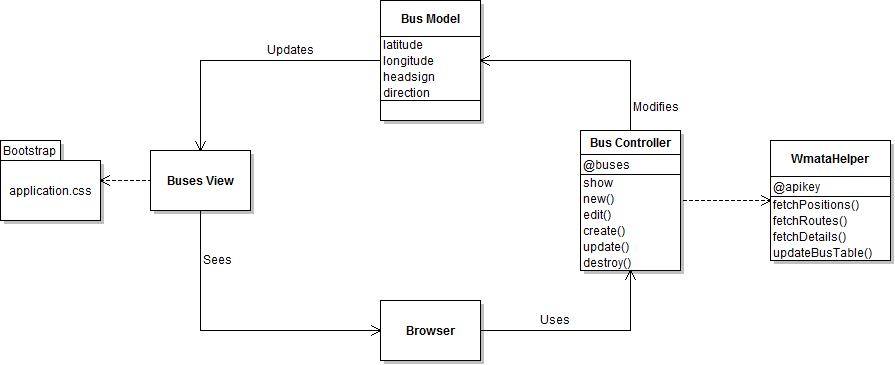
\includegraphics[scale=0.55]{busTrackerUML.png}}
	\caption{MVC control pattern}
	\label{fig:MVC}
\end{figure}

This MVC handles user requests in the following way.  If a request is sensed via the browser (from the user or an update timer), the controller is called and told to modify the model in some way.  When the model is changed, an update function is called for the View (usually through an observer) and the result is interpreted and rendered by the browser.  This cycle will repeat itself every time a user clicks on a controller action.  The important thing about this architecture is that it encapsulates the different components and the View never has access to the Model -- creating a scalable and secure system.\\

Another example of Rails favoring convention over configuration is shown in the controller.  Rails prefers to use RESTful URIs which correspond to HTTP's GET, POST, PUT, DELETE etc methods.  In Rails, these RESTful URIs are implemented via CRUD -- Create, Read, Operate Destroy.  Bus Tracker supports these CRUD operations as well and utilizes them to create local instances of each bus and any data associated with it.\\

Some of the API features, specific to Bus Tracker, are also listed in Figure \ref{fig:MVC}.  The controller relies on fetching data from the WMATA servers which  are accessed via a helper class - WmataHelper.  WmataHelper fetches all the possible information and then the required information is stored locally using the Controller's CRUD operations.  For example, a new bus can be made with the create() method and then assigned the data from the API call or an existing bus can have it's information updated with the update() method.  The locality reduces latency and WMATA server usage.  Another API that is being utilized in Bus Tracker is Twitter's Bootstrap which provides additional CSS options. Combining Bootstrap with the View can create dynamic web pages that can render correctly on phones or desktop computers with minimal overhead.

\subsection*{Model Relationships}

Bus Tracker will contain information regarding all the buses in the DC metro area which can be quite a lot at times.  The final model will consist of many relationships that tie the buses to physical locations on the map.  Figure \ref{fig:busEntity} shows the expected final relationship scheme for Bus Tracker.

\begin{figure}[ht]
	\centerline{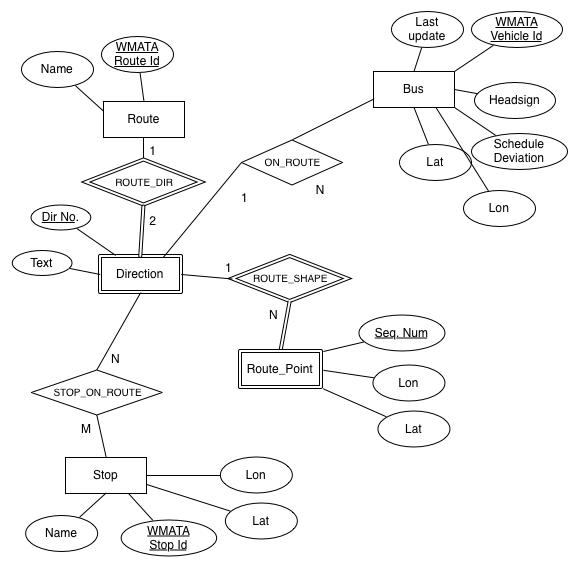
\includegraphics[scale=0.43]{bus-entity-rel.png}}
	\caption{Model relationship diagram}
	\label{fig:busEntity}
\end{figure}

This diagram shows the Bus model and all of the relationships necessary to provide a user with the best information available.  As a brief overview, each bus has certain characteristics regardless whether it is en route or not.  If the bus is en route, there is some more information needed such as what direction it is headed in, what route shape is displayed on the map, and what are the defining characteristics of the next stops.  This is the information that will be stored locally after retrieving the information from WMATA.

\subsection*{API integration}

To complete this project in a timely fashion, multiple APIs had to be utilized.  As mentioned before one of these APIs is from WMATA which pulls the bus information. Another API that is used to display the map itself and the data on the map is Google Maps.  Figure \ref{fig:designOverview} shows an overview for how these APIs connect to the web server.

\begin{figure}[ht]
	\centerline{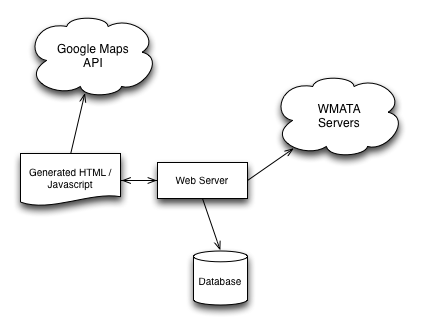
\includegraphics[scale=0.6]{design.png}}
	\caption{API integration overview}
	\label{fig:designOverview}
\end{figure}

The web server begins this process by sending a request to the WMATA servers.  Once the information is received, CRUD operations are used to store this information in a local PostgreSQL database.  This information is sent to the View and lastly rendered using the Google Maps API. Google Maps provides a unique interface which makes it possible to display coordinates for buses and their routes.  Figure \ref{fig:busSchema} shows how the information is pulled from the WMATA servers for display on the map.


\begin{figure}[ht]
	\centerline{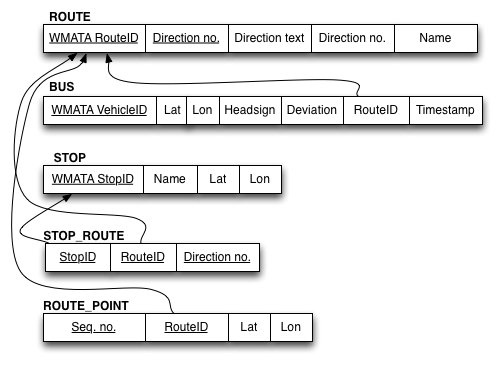
\includegraphics[scale=0.6]{bus-schema.png}}
	\caption{Schema for WMATA API}
	\label{fig:busSchema}
\end{figure}

Using this information, all the bus information can be connected back to a certain bus using the route ID.  The local database also mimics this structure to make the conversion easier.  

\section*{Task Breakdown and Timeline}
\begin{description}
	\item Tasks to be done by:  November 10, 2012  	
	
	\begin{enumerate}
		\item Initial rails setup [Cluck]
		\item CSS styling using twitter bootstrap [Cluck]
		\item Display map on index page [Cluck]
		\item Fetch bus positions from WMATA servers [Will]
		\item Store WMATA response in database [Will]
		\item Draw markers on map for bus locations [Will]
		\item Draw lines on map for bus routes [Will]
		\item Display initial map area based on geolocation reading [Cluck]
		\item Show info window when bus marker is clicked, including the following [Will]
		\begin{enumerate}
			\item Route name
			\item Schedule deviation (lateness)
			\item Time of last position update (data staleness)
			\item Headsign
			\item Direction
		\end{enumerate}
	\end{enumerate}
	\item Tasks to be done by: November 20, 2012
	\begin{enumerate}
		\item Fetch routes from WMATA servers [Will]
		\item Fetch stops from WMATA servers [Will]
		\item Store routes in database [Cluck]
		\item Store stops in database [Cluck]
		\item Layer toggle widget that shows Google traffic overlay, bus markers, and stop markers [Will]
	\end{enumerate}
	\item Tasks to be done by: December 3, 2012
	\begin{enumerate}
		\item Display bus stops with markers on map [Cluck]
		\item Control WMATA polling to avoid exceeding usage limits [Will]
		\item Show info window when stop marker is clicked [Will]
			\begin{enumerate}
				\item Show which routes and directions the use the stop
				\item Show next bus wait time projections for each route that uses the stop
			\end{enumerate}
		\item Add iOS/Android functionality using mobile web browser [Cluck]
	\end{enumerate}
\end{description}
\end{document}

